\newpage{}
\section{Appendix}
\label{sec:appendix}

\subsection{Base Models of Varying Sizes and Architectures}
\label{sec:70b_microbenchmark}

\begin{figure}[h]
    \centering
    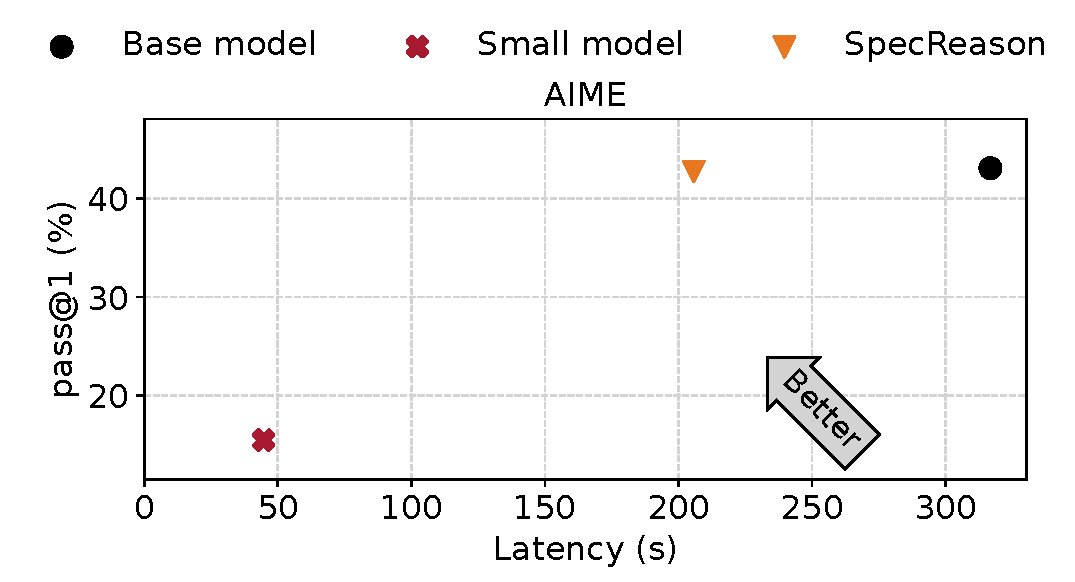
\includegraphics[width=0.6\textwidth]{figures/70b_results.pdf}
    \caption{\name{}'s results on the model combination (R1-70B, R1-1.5B).}
    \label{fig:70b_results}
\end{figure}




To demonstrate the generality of \name{}, we replace the QwQ-32B base model with DeepSeek's R1-70B and evaluate on the same representative subdatasets as in~\S\ref{sec:acc_lat_tradeoff}. Given the size of the R1-70B model, we deploy it across four A100-80GB GPUs using a tensor parallelism degree of 4.

On the AIME subdataset, \name{} achieves a 1.5$\times$ latency reduction compared to vanilla R1-70B inference. This speedup is smaller than the gains observed with the QwQ-32B model in our main results (1.9$\times$) due to two key factors. First, the R1-70B model benefits from both stronger hardware and greater parallelism (4-way TP on A100s), resulting in a 1.5$\times$ lower time-per-token (TPT) compared to QwQ-32B (2-way TP on A6000s). In contrast, the smaller model R1-1.5B sees only a modest 1.1$\times$ TPT improvement on stronger hardware, which narrows the performance gap between base and small models and thus diminishes latency savings. Second, QwQ-32B is empirically a stronger model -- outperforming R1-70B across many reasoning benchmarks~\cite{qwq_32b} -- and this performance gap impacts their respective abilities to assess intermediate steps. To maintain accuracy, we adopt a stricter acceptance threshold when using R1-70B as the base model, which reduces the fraction of steps offloaded to the small model (23.2\% compared to 40.8\% in the main results).

\subsection{Intuition behind Accuracy Improvement}

\begin{figure}[h]
    \centering
    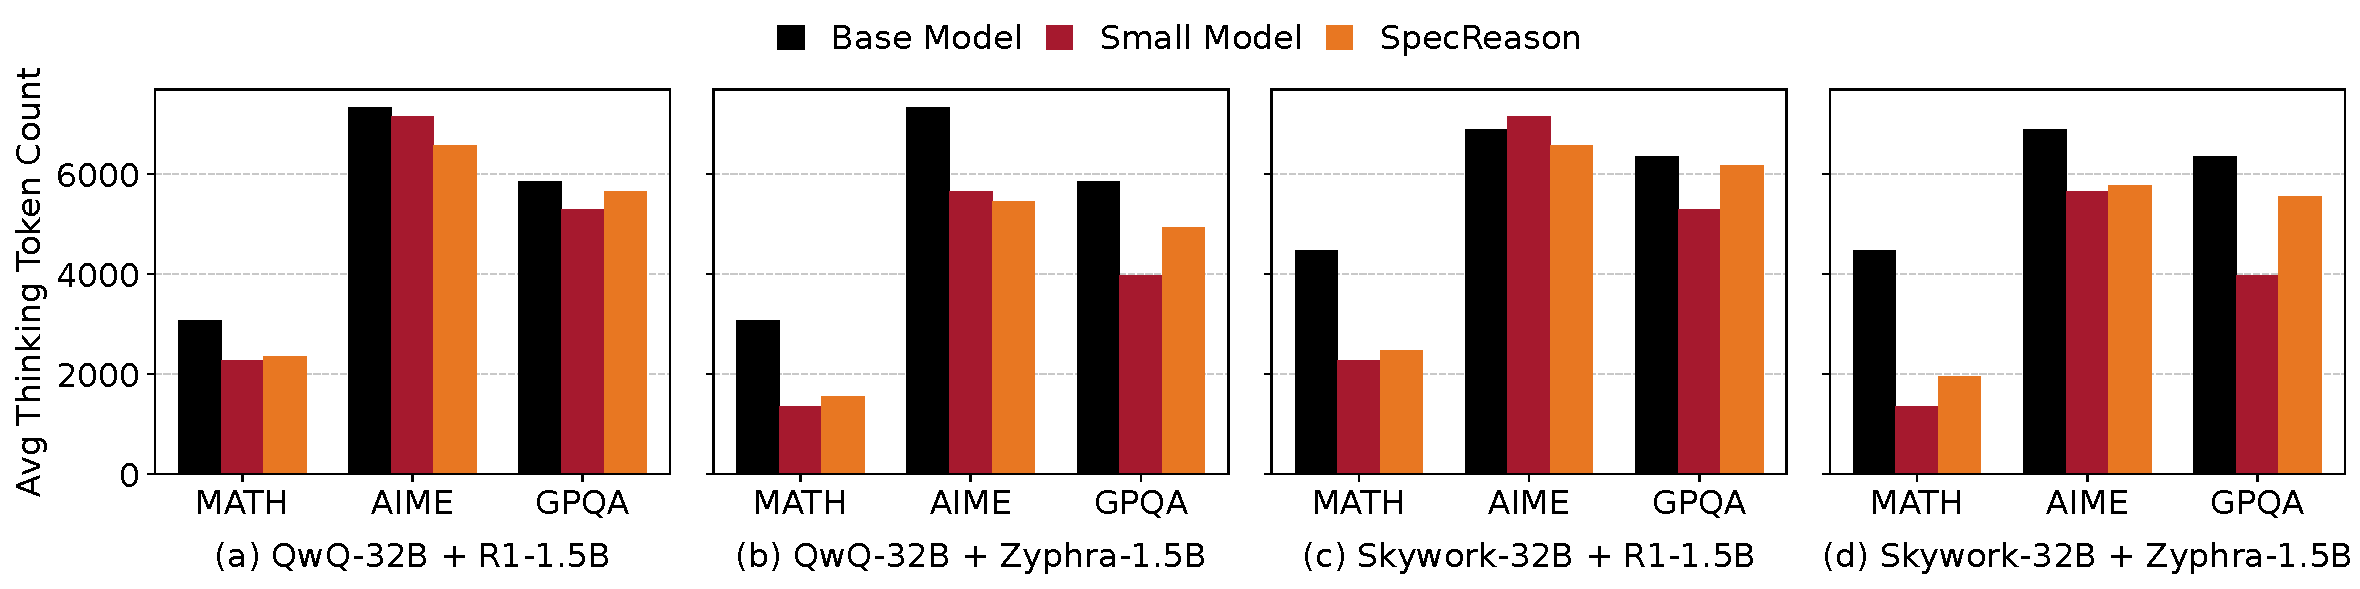
\includegraphics[width=0.99\textwidth]{figures/acc_insight_len_all.pdf}
    \caption{Intuition behind \name{}'s accuracy improvement on all datasets and model combinations.}
    \label{fig:acc_insight_len_all}
\end{figure}

In Fig.~\ref{fig:acc_insight_len_all}, we evaluate the average thinking token count of \name{} and two vanilla inference baselines on a wide range of datasets and model combinations. We observe that the small model is generally less verbose than the base model, and because \name{} adopts many speculated steps from the small model, its token consumption is reduced by $1.0-1.3\times$, $1.2-2.0\times$, $1.0-1.8\times$, and $1.1-2.3\times$ on the four model combinations, respectively.
